% Options for packages loaded elsewhere
\PassOptionsToPackage{unicode}{hyperref}
\PassOptionsToPackage{hyphens}{url}
\PassOptionsToPackage{space}{xeCJK}
%
\documentclass[
  11pt,
  letterpaper,
]{article}
\usepackage{lmodern}
\usepackage{amssymb,amsmath}
\usepackage{ifxetex,ifluatex}
\ifnum 0\ifxetex 1\fi\ifluatex 1\fi=0 % if pdftex
  \usepackage[T1]{fontenc}
  \usepackage[utf8]{inputenc}
  \usepackage{textcomp} % provide euro and other symbols
\else % if luatex or xetex
  \usepackage{unicode-math}
  \defaultfontfeatures{Scale=MatchLowercase}
  \defaultfontfeatures[\rmfamily]{Ligatures=TeX,Scale=1}
  \ifxetex
    \usepackage{xeCJK}
    \setCJKmainfont[]{Noto Sans CJK TC Medium}
  \fi
  \ifluatex
    \usepackage[]{luatexja-fontspec}
    \setmainjfont[]{Noto Sans CJK TC Medium}
  \fi
\fi
% Use upquote if available, for straight quotes in verbatim environments
\IfFileExists{upquote.sty}{\usepackage{upquote}}{}
\IfFileExists{microtype.sty}{% use microtype if available
  \usepackage[]{microtype}
  \UseMicrotypeSet[protrusion]{basicmath} % disable protrusion for tt fonts
}{}
\makeatletter
\@ifundefined{KOMAClassName}{% if non-KOMA class
  \IfFileExists{parskip.sty}{%
    \usepackage{parskip}
  }{% else
    \setlength{\parindent}{0pt}
    \setlength{\parskip}{6pt plus 2pt minus 1pt}}
}{% if KOMA class
  \KOMAoptions{parskip=half}}
\makeatother
\usepackage{xcolor}
\IfFileExists{xurl.sty}{\usepackage{xurl}}{} % add URL line breaks if available
\IfFileExists{bookmark.sty}{\usepackage{bookmark}}{\usepackage{hyperref}}
\hypersetup{
  hidelinks,
  pdfcreator={LaTeX via pandoc}}
\urlstyle{same} % disable monospaced font for URLs
\usepackage[margin=0.75in]{geometry}
\usepackage{graphicx}
\makeatletter
\def\maxwidth{\ifdim\Gin@nat@width>\linewidth\linewidth\else\Gin@nat@width\fi}
\def\maxheight{\ifdim\Gin@nat@height>\textheight\textheight\else\Gin@nat@height\fi}
\makeatother
% Scale images if necessary, so that they will not overflow the page
% margins by default, and it is still possible to overwrite the defaults
% using explicit options in \includegraphics[width, height, ...]{}
\setkeys{Gin}{width=\maxwidth,height=\maxheight,keepaspectratio}
% Set default figure placement to htbp
\makeatletter
\def\fps@figure{htbp}
\makeatother
\setlength{\emergencystretch}{3em} % prevent overfull lines
\providecommand{\tightlist}{%
  \setlength{\itemsep}{0pt}\setlength{\parskip}{0pt}}
\setcounter{secnumdepth}{-\maxdimen} % remove section numbering

\setCJKmonofont{Noto Sans Mono CJK TC}


\author{}
\date{}

\begin{document}

\hypertarget{a-physics-inspired-computational-approach-to-chinese-character-analysis-network-patterns-and-semantic-evolution}{%
\section{A Physics-Inspired Computational Approach to Chinese Character
Analysis: Network Patterns and Semantic
Evolution}\label{a-physics-inspired-computational-approach-to-chinese-character-analysis-network-patterns-and-semantic-evolution}}

Wen G. Gong*

*Corresponding author: digital-duck@outlook.com

2025-01-01

\hypertarget{abstract}{%
\subsection{Abstract}\label{abstract}}

This paper presents a novel perspective on Chinese characters as a
naturally evolved system for encoding and transmitting concepts and
meaning, following universal principles of organization and growth. By
treating character components as fundamental elements that interact
through ``semantic forces'', we develop a systematic framework that
reveals how Chinese writing mirrors patterns found throughout nature.
The approach integrates physics principles, computational analysis, and
traditional understanding to demonstrate how characters emerge from
elemental characters (元字) through natural combination patterns,
similar to physical and biological systems. Using the Fibonacci sequence
as an organizing principle, we show how approximately 3,000 Chinese
characters can be systematically understood through their evolutionary
patterns. Our computational implementation, ZiNets (字网), provides
evidence for this perspective by revealing recurring patterns of
character composition and semantic development.

\hypertarget{disclaimer}{%
\subsection{Disclaimer}\label{disclaimer}}

A more accessible title for this paper might be \textbf{``A Reductionist
Approach to Simplify Learning Chinese Characters''}, as the author is
not a professional researcher in the fields of physics, computational
linguistics, or Chinese language studies. However, with a deep interest
in understanding Chinese characters (汉字), the author wishes to share
this interdisciplinary exploration aimed at simplifying the learning
process.

Terms such as \textbf{``physics,'' ``structure,'' ``interaction,''
``force,'' ``emergence,''} and \textbf{``Fibonacci sequence''} are used
heuristically and metaphorically to inspire new ways of thinking about
Chinese characters. In the computational approach, terms like
\textbf{``data structure,'' ``node,''} and \textbf{``component''} often
represent ``structure'' in physics; \textbf{``relationship''} and
\textbf{``link''} represent ``interaction'' or ``force'' in physics; and
\textbf{``network''} and \textbf{``system''} represent ``complex
matter'' in physics.

The author sincerely welcomes \textbf{criticism, feedback, and
suggestions} to further our collective understanding of Chinese
characters and improve the framework presented here.

\hypertarget{introduction}{%
\subsection{1. Introduction}\label{introduction}}

Chinese characters {[}1{]}, as one of the oldest continuously used
writing systems, present a unique opportunity for studying how symbolic
systems naturally evolve to encode and transmit meaning.

Traditional Chinese linguistics classifies characters into six
categories (六书) based on their formation principles:

\begin{itemize}
\item
  Pictograms (象形): Direct pictorial representations of concrete
  objects, forming the earliest character set. Examples include 日
  (sun), 月 (moon), 山 (mountain), and 人 (human).
\item
  Simple Ideograms (指事): Abstract concepts represented through
  symbolic forms or modified pictograms. Examples include 上 (above), 下
  (below), 一 (one), and 二 (two).
\item
  Compound Ideograms (会意): Logical combinations of two or more
  pictograms or ideograms to create new meanings. For instance, 休
  (rest) shows a 人 (person) leaning against a 木 (tree), while 明
  (bright) combines 日 (sun) and 月 (moon).
\item
  Phono-semantic Compounds (形声): The most prevalent type, combining a
  semantic component (meaning indicator) with a phonetic component
  (pronunciation guide). Examples include 妈 (mother; semantic: 女
  woman, phonetic: 马) and 湖 (lake; semantic: 氵water, phonetic: 胡
  hu).
\item
  Transfer Characters (转注): A debated category describing characters
  with extended or adapted meanings.
\item
  Loan Characters (假借): Characters borrowed phonetically to represent
  words with similar pronunciations.
\end{itemize}

While extensive research exists on the structural evolution of Chinese
characters through various writing styles {[}2{]} - ranging from Oracle
Bone Script (甲骨文), Bronze Script (金文), Seal Script (篆书), Clerical
Script (隶书), Regular Script (楷书), Semi-cursive Script (行书), to
Cursive Script (草书), traditional scholarship has primarily focused on
their morphological aspects. This paper proposes a novel perspective:
Chinese characters represent a naturally evolved system that follows
universal principles of organization and growth observed throughout
nature.

Key insights: - Chinese characters evolved as a coherent conceptual
encoding system through natural principles rather than arbitrary design
- Character formation patterns parallel physical and biological growth
processes - The system exhibits self-organization and natural evolution
characteristics - Computational analysis reveals systematic patterns in
character composition

Our physics-inspired framework demonstrates: - Natural combinatorial
patterns in elemental characters (元字) - Fibonacci-like growth
sequences in character complexity - Stable semantic structures emerging
from component interactions - System coherence maintained through
evolutionary development

\hypertarget{methodology}{%
\subsection{2. Methodology}\label{methodology}}

\hypertarget{the-concept-of-elemental-characters-ux5143ux5b57}{%
\subsubsection{2.1 The Concept of Elemental Characters
(元字)}\label{the-concept-of-elemental-characters-ux5143ux5b57}}

Unlike traditional radical classification systems that focus primarily
on handwriting and structural organization, we introduce the concept of
元字 (elemental characters) as fundamental semantic building blocks,
expanding on radicals and phonetic components. These approximately
300-400 elemental characters serve as the ``periodic table'' of Chinese
characters, each carrying independent semantic meaning that contributes
to the formation of more complex characters. They may not always look as
simple as pictograph, but carry distinct conceptual meaning and
semantics.

Key characteristics:

\begin{itemize}
\tightlist
\item
  Semantic Independence: Each 元字 carries its own primitive, meaningful
  concept (e.g., 乐 for music/happiness)
\item
  Combinatorial Power: They combine to form more complex characters
  following semantic and structural rules
\item
  Frequency Patterns: Their usage follows natural distribution patterns
  in character formation
\item
  Cross-Category Utility: They often participate in multiple semantic
  domains
\end{itemize}

This approach differs from the traditional radical system in several key
ways:

\begin{itemize}
\tightlist
\item
  Focus on meaning rather than just writing structure
\item
  Inclusion of semantically significant characters that aren't
  traditional radicals
\item
  Emphasis on combinatorial patterns rather than categorization
\item
  Recognition of independent semantic value
\end{itemize}

\hypertarget{spatial-framework-and-component-interactions}{%
\subsubsection{2.2 Spatial Framework and Component
Interactions}\label{spatial-framework-and-component-interactions}}

Our physics-inspired approach treats Chinese character composition as a
system of components interacting within a well-defined spatial
framework:

\begin{itemize}
\tightlist
\item
  Coordinate Space (九字宫 Enhancement)

  \begin{itemize}
  \tightlist
  \item
    The traditional nine-grid system serves as a ``coordinate space''
    for component positioning designed for calligraphy.
  \item
    Components interact across specific positions, similar to particle
    interactions in physics
  \item
    Additional dimensions (mid-inner, mid-outer) handle enclosure
    structures, analogous to how physics adds dimensions to describe
    complex systems
  \end{itemize}
\item
  Topological Patterns

  \begin{itemize}
  \tightlist
  \item
    Irreducible patterns: independent components like pictograph
    characters (e.g.~日,月,人)
  \item
    Linear arrangements: Components interact in sequential positions
    (e.g., 明, 街, 尖, 曼)
  \item
    Enclosure patterns: Outer components create boundary conditions for
    inner elements (e.g.~回)
  \item
    Triangle patterns: components arranged in triangular positions
    (e.g.~品, 森)
  \item
    Quadrant patterns: components arranged in square positions
    (e.g.~疑,叕)
  \item
    Nested structures: Multiple levels of containment create
    hierarchical relationships (e.g.~藻)
  \end{itemize}
\item
  Special Case Handling

  \begin{itemize}
  \tightlist
  \item
    Enclosure characters (回, 国) utilize extended spatial dimensions
  \item
    Mid-inner position represents contained elements
  \item
    Mid-outer position represents containing elements
  \end{itemize}
\end{itemize}

\hypertarget{fibonacci-organization-and-ux5143ux5b57-emergence}{%
\subsubsection{2.3 Fibonacci Organization and 元字
Emergence}\label{fibonacci-organization-and-ux5143ux5b57-emergence}}

The Fibonacci sequence (1, 1, 2, 3, 5, 8, 13, 21, 34, 55, \ldots)
naturally emerges in growth patterns throughout nature. When visualized,
it creates an elegant spiral known as the golden spiral, seen in
countless natural forms - from the arrangement of sunflower seeds to the
shell of a nautilus. This pattern represents nature's efficient approach
to growth and organization, where complex structures build upon simpler
foundations in a harmonious and balanced way {[}3{]}.

\begin{figure}
\centering
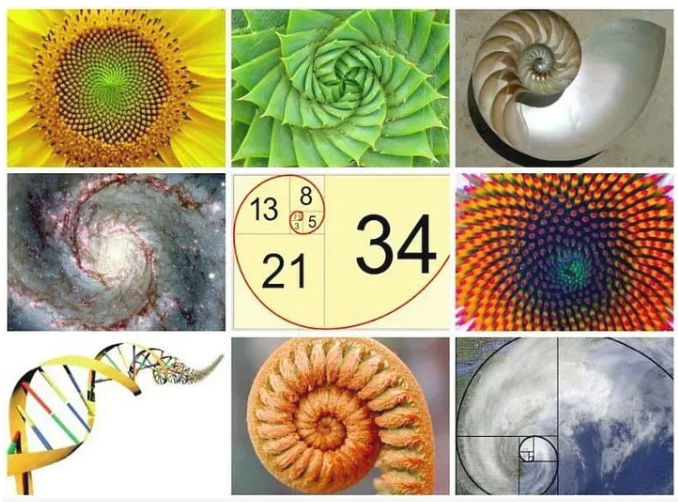
\includegraphics{./images/fibonacci-spiral.png}
\caption{fibonacci-spiral}
\end{figure}

We borrow the Fibonacci sequence to organize Chinese characters in a
similar natural progression: from simple pictographs to sophisticated
composite characters, from concrete objects to abstract concepts. Just
as the Fibonacci spiral demonstrates how complex natural patterns emerge
from simple mathematical relationships, our organization reveals how
Chinese writing evolved from basic elements (元字) into increasingly
complex expressions. Each level introduces new fundamental characters
that, like the expanding spiral, serve as building blocks for richer
linguistic representations. This approach mirrors nature's own
efficiency in developing complex systems from simple foundations.

In the following, we list the first 8 sets of 元字 families. Traditional
radicals with independent meaning are noted under ``Radical form
mapping'' (e.g.~灬 means fire).

\begin{itemize}
\item
  1 (一): 气 (primordial force/energy)

  \begin{itemize}
  \tightlist
  \item
    The most fundamental 元字
  \item
    Represents the emergence of invisible form from formlessness
    (无中生有)
  \item
    Base unit for energy and force concepts
  \item
    炁 is an uncommon and old form for 气, rarely used. But its lower
    radical (灬) hints its semantic meaning related to fire and energy.
  \end{itemize}
\item
  1 (一): 点,线 (primitive low-dimensional object)

  \begin{itemize}
  \tightlist
  \item
    Basic radicals 元字: 丶(dot), 一 (horizontal line), 丨 (vertical
    line), 丿 (north-east line), 乀 (south-east line)
  \item
    Represents visible simple form (i.e., point- or line-like objects)
  \end{itemize}
\item
  2 (二): 日,月 (sun and moon)

  \begin{itemize}
  \tightlist
  \item
    First pair of naturally contrasting 元字
  \item
    Represents 2 visible solar objects and a fundamental abstraction in
    the basic dualism philosophy (阴阳)
  \item
    Foundation for temporal and luminance concepts
  \item
    Both characters can be used as radicals. It is worthwhile to note
    that 月 means body part meat/flesh 肉 when used as radical. This is
    likely a historical coincidence where 月 was adopted as the
    simplified writing form for 肉.
  \end{itemize}
\item
  3 (三): 天,地,人 (heaven, earth, human)

  \begin{itemize}
  \tightlist
  \item
    Tripartite domain 元字
  \item
    Establishes basic spatial and existential framework for human
    cognitive psychic
  \item
    Core reference for positioning and relationships
  \item
    Radical form mapping: 土 for 地, 亻for 人.
  \end{itemize}

  \begin{figure}
  \centering
  
\includegraphics{./images/sun-moon-heaven-human-earth-meditation-morning.jpg}
  \caption{Heaven-Earth-Human}
  \end{figure}

  This AI generated image {[}4{]} embodies 6 元字 (气,日,月,天,地,人) in
  an integrated visual representation.
\item
  5 (五): 金,木,水,火,土 (metal, wood, water, fire, earth)

  \begin{itemize}
  \tightlist
  \item
    Material phase 元字
  \item
    Fundamental 5 elements (五行) for describing physical and
    materialistic world in ancient philosophy.
  \item
    Base components for nature-related characters
  \item
    Radical form mapping: 钅for 金, 氵冫for 水, 灬 for 火, 木, 土 are
    often rended in narrower form when used as radicals. The semantic
    meanings are the same.
  \end{itemize}
\item
  8 (八): 东,南,西,北,春,夏,秋,冬 (directions and seasons)

  \begin{itemize}
  \tightlist
  \item
    Spatiotemporal 元字
  \item
    Complete system of orientation and cyclical change
  \item
    Foundation for location and time-based concepts
  \end{itemize}
\item
  13 (十三): 生,鼠,牛,虎,兔,龙,蛇,马,羊,猴,鸡,狗,猪 (basic life forms
  expressed in 12 Zodiac animals)

  \begin{itemize}
  \tightlist
  \item
    Biological object 元字
  \item
    Complex natural phenomena
  \item
    Base set for describing living things
  \item
    Radical form mapping: 牜for 牛, 虫 is a radical for 蛇 and other
    insects, 犭is a radical for many animals (e.g.~猴,狗,猪), 羊,⺶,⺷
    are variant radical forms for 羊(Sheep), radical for 马 appears
    narrower.
  \end{itemize}
\item
  21 (二十一): Quantification and Measurement 元字

  \begin{itemize}
  \tightlist
  \item
    Numerical System (15 characters):

    \begin{itemize}
    \tightlist
    \item
      Basic numerals: 一,二,三,四,五,六,七,八,九,十
    \item
      Large quantities: 百,千,万,亿,零
    \item
      These form the foundation for all quantitative description
    \end{itemize}
  \item
    Physical Units (6 characters):

    \begin{itemize}
    \tightlist
    \item
      Time measurement: 秒,分,时

      \begin{itemize}
      \tightlist
      \item
        Progression from smallest (second) to largest (hour)
      \item
        Reflects natural cycles and human activity patterns
      \end{itemize}
    \item
      Length measurement: 寸,丈,里

      \begin{itemize}
      \tightlist
      \item
        Traditional Chinese units of length
      \item
        Scales from human body reference (寸) to geographic distance
        (里)
      \end{itemize}
    \end{itemize}
  \end{itemize}
\end{itemize}

This set represents the emergence of systematic measurement and
counting.

\begin{itemize}
\tightlist
\item
  34 (三十四): Human Form and Action 元字

  \begin{itemize}
  \tightlist
  \item
    Basic parts:
    心(忄),头,首,面,口,目,眉,鼻,耳,舌,牙,齿,手(扌),又,足,血,肉,身,尸,骨,皮,毛(彡)
  \item
    Action indicators: 言(讠),口, 看,听,思,食(饣),走(辶),立
  \item
    Identity: 男,女,子,自,己
  \item
    Radical form mapping: 忄for 心, 扌for 手, 辶 for 足, 讠for 言, 饣for
    食, often (not always) in action context, e.g.~emotional thinking,
    holding, walking, communicating, respectively. 目, 口, 足, 骨, 耳
    appear as radicals too. Some of these characters (like 首, 面) can
    function as both nouns (head, face) and measure words/classifiers in
    different contexts.
  \end{itemize}
\end{itemize}

This set introduces fundamental components for describing human
existence and behavior.

\hypertarget{pattern-discovery-and-physical-analogies}{%
\subsubsection{2.4 Pattern Discovery and Physical
Analogies}\label{pattern-discovery-and-physical-analogies}}

The systematic analysis of character composition through our spatial
framework reveals several key patterns that parallel physical systems:

\begin{itemize}
\tightlist
\item
  Compositional Rules as Interaction Laws

  \begin{itemize}
  \tightlist
  \item
    Just as physical particles interact according to fundamental forces,
    character components combine following specific spatial and semantic
    rules
  \item
    The nine-grid system acts as a ``field'' where components interact
    to form stable configurations
  \item
    Component positions influence each other, similar to how particles
    create and respond to fields
  \end{itemize}
\item
  Emergent Patterns

  \begin{itemize}
  \tightlist
  \item
    Regular combinations: Certain components frequently appear in
    specific relative positions
  \item
    Stability patterns: Some configurations appear more frequently in
    the character set, suggesting ``stable states''
  \item
    Conservation laws: Semantic meaning is preserved across different
    spatial arrangements
  \end{itemize}
\item
  Hierarchical Organization

  \begin{itemize}
  \tightlist
  \item
    Like physical systems exhibiting different scales of organization,
    characters show multiple levels of structure
  \item
    Local interactions (between adjacent components) lead to global
    patterns
  \item
    Complex characters emerge from simpler stable configurations
  \end{itemize}
\end{itemize}

\hypertarget{results}{%
\subsection{3. Results}\label{results}}

\hypertarget{web-application-implementation-zinets-ux5b57ux7f51}{%
\subsubsection{3.1 Web Application Implementation: ZiNets
(字网)}\label{web-application-implementation-zinets-ux5b57ux7f51}}

Our web-based visualization tool, ZiNets (Zi Network System), implements
the theoretical framework through an interactive character decomposition
system. The name ``ZiNets'' reflects its primary function:
reconstructing Chinese characters (Zi, 字) into networks of their
elemental components.

\hypertarget{character-decomposition-visualization}{%
\paragraph{3.1.1 Character Decomposition
Visualization}\label{character-decomposition-visualization}}

\begin{figure}
\centering
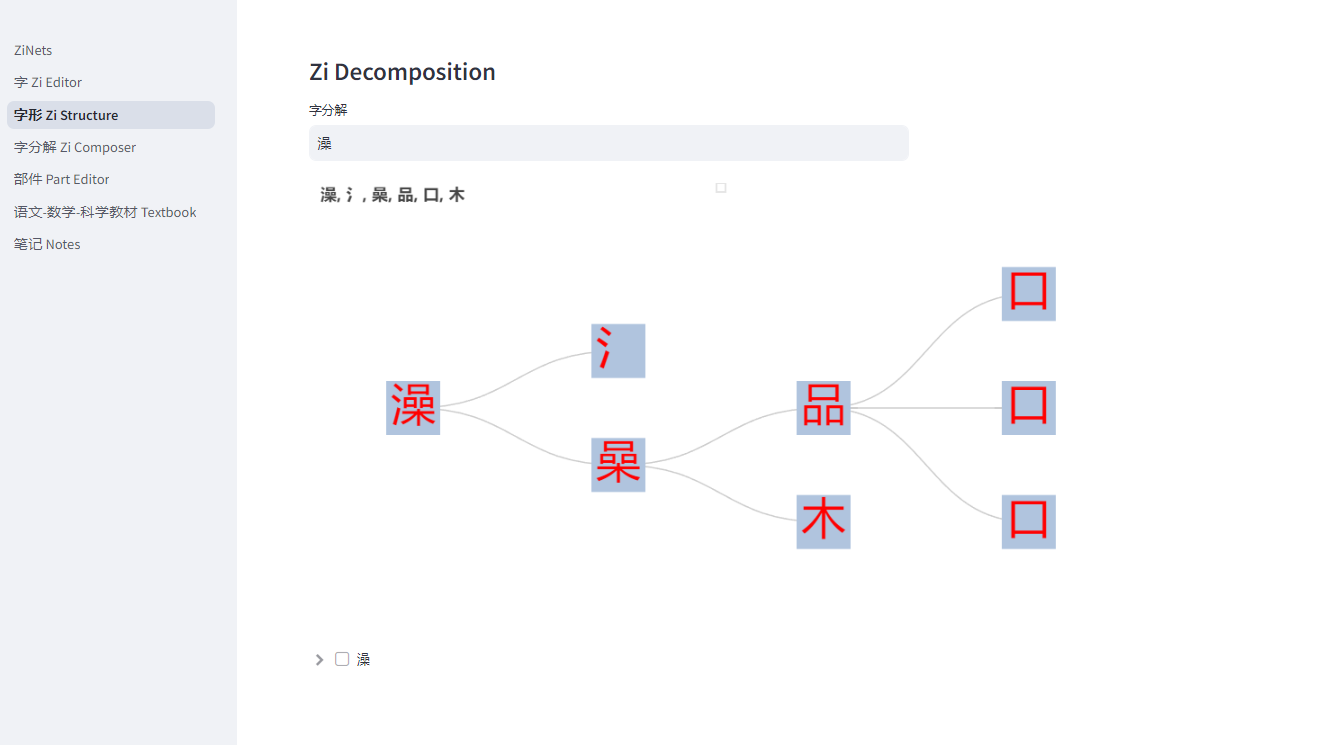
\includegraphics{./images/app_decomposing-zi.png}
\caption{Zi Network Pattern}
\end{figure}

The core feature of ZiNets is its hierarchical decomposition
visualization:

\begin{itemize}
\tightlist
\item
  Network Structure

  \begin{itemize}
  \tightlist
  \item
    Characters are represented as nodes in a directed graph
  \item
    Decomposition relationships are shown as edges
  \item
    Left-to-right layout reflects decomposition hierarchy
  \item
    Visual clarity maintained through spatial organization
  \end{itemize}
\item
  Hierarchical Analysis

  \begin{itemize}
  \tightlist
  \item
    Multiple levels of decomposition shown simultaneously
  \item
    Clear parent-child relationships between components
  \item
    Preservation of structural relationships
  \item
    Explicit visualization of component reuse
  \end{itemize}
\item
  Component Identification

  \begin{itemize}
  \tightlist
  \item
    Each 元字 and component clearly bounded
  \item
    Consistent visual representation of elements
  \item
    Immediate recognition of basic building blocks
  \item
    Clear distinction between levels of composition
  \end{itemize}
\end{itemize}

\hypertarget{frequency-analysis-and-natural-efficiency}{%
\subsubsection{3.2 Frequency Analysis and Natural
Efficiency}\label{frequency-analysis-and-natural-efficiency}}

Our computational analysis of approximately 3,000 commonly used HSK
Chinese characters {[}5{]} reveals striking patterns in 元字 usage that
demonstrate natural optimization principles:

\begin{itemize}
\item
  Distribution of High-frequency Elements (\textgreater100 occurrences):

  The table presents the 25 most frequently used elemental
  characters/radicals in commonly used Chinese characters. These
  elements primarily belong to the 2nd (日,月), 3rd (天地人) and 4th
  (金木水火土) Fibonacci sequence number sets. While 气 (air/energy) is
  not present in this list, its conceptual force permeates the character
  system. The distribution pattern suggests a natural evolution toward
  efficient structural components, with elements grouped into distinct
  semantic categories:

  \begin{itemize}
  \tightlist
  \item
    Heaven-related elements (天界): 日, 月
  \item
    Human-related elements (人类): 口, 女, 人(亻), 心 (忄), 目, 手(扌),
    辶
  \item
    Natural elements (自然):

    \begin{itemize}
    \tightlist
    \item
      Five elements (五行): 金(钅), 木, 水(氵), 火, 土
    \item
      Earth variations: 阝, 艹, 纟
    \item
      Living beings (生物): 虫, 鸟, 马
    \end{itemize}
  \end{itemize}

  \begin{figure}
  \centering
  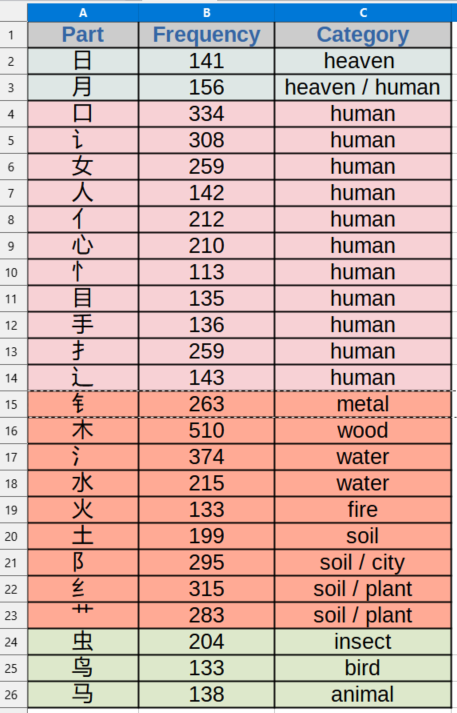
\includegraphics{./images/part-frequency-top-25.png}
  \caption{top-25-elemental-character-set}
  \end{figure}
\item
  Semantic Distribution

  \begin{itemize}
  \tightlist
  \item
    Predominance of earth and nature elements
  \item
    High representation of human-related components
  \item
    Progressive development from concrete to abstract concepts
  \item
    Clear conceptual hierarchy from physical to abstract domains
  \end{itemize}
\item
  Efficiency Characteristics

  \begin{itemize}
  \tightlist
  \item
    Core 元字 function as versatile semantic foundations
  \item
    System balances complexity with expressive power
  \item
    High-frequency components span fundamental categories
  \item
    Evidence of evolutionary selection for optimal semantic encoding
  \end{itemize}
\end{itemize}

\hypertarget{case-studies---composite-characters}{%
\subsubsection{3.3 Case Studies - Composite
Characters}\label{case-studies---composite-characters}}

\hypertarget{the-ux65e5-family}{%
\paragraph{3.3.1 The 日 Family}\label{the-ux65e5-family}}

\begin{figure}
\centering
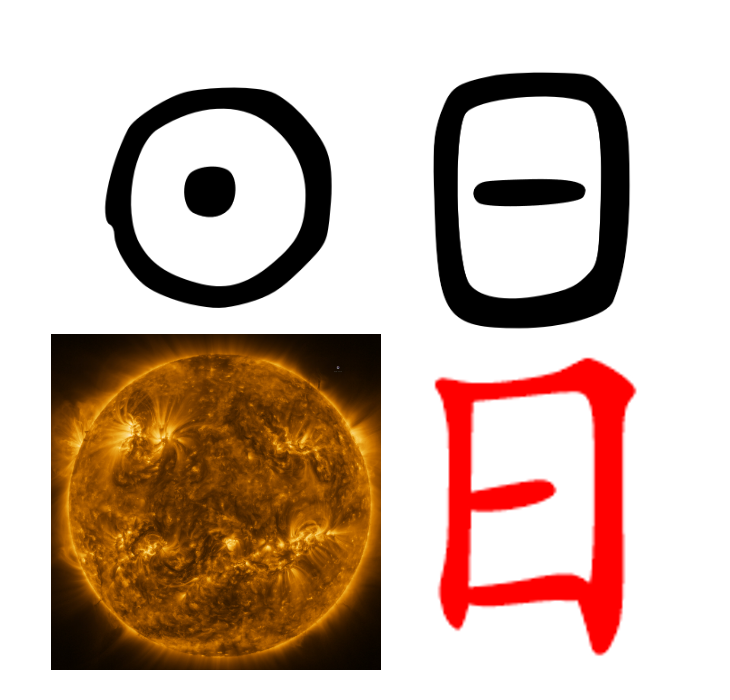
\includegraphics{./images/zi_sun.png}
\caption{zi\_sun}
\end{figure}

The Chinese character ``日'' (rì), meaning ``sun'' or ``day'', serves as
a powerful illustration of how Chinese characters efficiently encode
meaning, knowledge and wisdom. By examining composite characters that
incorporate ``日'', we gain insight into the profound ways in which the
written language captures essential truths and observations about the
world. These simple formulas provide a peek into the rich semantics of
the Chinese language. Consider the following examples:

\begin{itemize}
\item
  日 + 月 = 明 (míng):

  In early civilizations, the sun and moon were the primary sources of
  illumination. The combination of these two characters to form 明,
  meaning ``bright'' or ``clear'', elegantly captures this fundamental
  truth.
\item
  日 + 正 = 是 (shì):

  When the sun is directly overhead, it casts no shadows. This character
  combination, meaning ``is/to be'', extends the concept to seeing
  things clearly and objectively, free from distortion. The phrase
  ``实事求是'' (shíshìqiúshì) embodies this, urging us to seek truth
  through facts.
\item
  知 + 日 = 智 (zhì):

  The character 智, signifying wisdom or knowledge, combines ``to know''
  (知) with ``sun'' (日). This encapsulates the idea that true wisdom
  comes from understanding the way of the sun - selflessly radiating
  light and energy without expectation of reward.
\item
  日 + 日 + 日 = 晶 (jīng):

  The repetition of ``日'' intensifies the concept of brightness,
  resulting in a character that means ``crystal'' or ``bright and
  clear.'' This character beautifully captures the essence of a
  crystal's luminosity and transparency.
\item
  门 + 日 = 间 (jiān):

  When light shines through a doorway, it illuminates the space or
  interval between the door frames. This character cleverly represents
  the idea of a gap, space, or interval by combining the symbols for
  ``door'' and ``sun.''
\item
  日 + 寸 = 时 (shí):

  In ancient times, sundials were used to measure time by tracking the
  length and position of the sun's shadow. This character combines
  ``sun'' and ``inch,'' illustrating the concept of time through the
  metaphor of the sun's movement.
\item
  日 + 生 = 星 (xīng):

  The character for ``star'' combines ``sun'' and ``to be born'' or ``to
  produce,'' suggesting that stars are born from the sun or are suns
  themselves. This character reflects the ancient understanding of the
  connection between the sun and the celestial bodies in the sky.
\item
  丿 + 日 = 白 (bái):

  The character for ``white'' combines a stroke (丿) with the sun (日).
  This represents the scientific understanding that sunlight is composed
  of all colors, as demonstrated by Newton's prism experiment. The white
  appearance of sunlight is a result of the combination of all colors in
  the visible spectrum.
\item
  日 + 一 = 旦 (dàn):

  This character combines the sun with the horizontal stroke
  representing the horizon, capturing the moment when the sun rises
  above the earth's horizon at dawn. It signifies the beginning of a new
  day or cycle, as in ``元旦'' (New Year's Day).
\item
  九 + 日 = 旭 (xù):

  The character for ``rising sun'' or ``bright and splendid'' combines
  the symbol for the number nine (i.e.~many) with the sun. The idea of
  nine suns shining together evokes an image of unimaginable brightness
  and intensity.
\item
  日 + 十 = 早 (zǎo):

  Here, the sun is shown above a symbol resembling a treetop, indicating
  the early morning hours when the sun has risen above the trees. This
  character encapsulates the concept of ``early'' or ``morning.''
\item
  日 + 干 = 旱 (hàn):

  The combination of the sun and the character for ``dry'' or ``to dry''
  creates a character meaning ``drought.'' This illustrates the
  cause-and-effect relationship between intense sunlight and the drying
  out of the land, leading to drought conditions.
\end{itemize}

These examples barely scratch the surface, but this family demonstrates
how Chinese characters, through their composition, reveals profound
insights and encodes knowledge in a uniquely efficient manner unmatched
by other writing systems. Children learning Chinese characters are
exposed to basic scientific concepts and knowledge while mastering the
language, a feature not found in many other languages.

\hypertarget{the-ux79ba-family}{%
\paragraph{3.3.2 The 禺 Family}\label{the-ux79ba-family}}

\begin{figure}
\centering
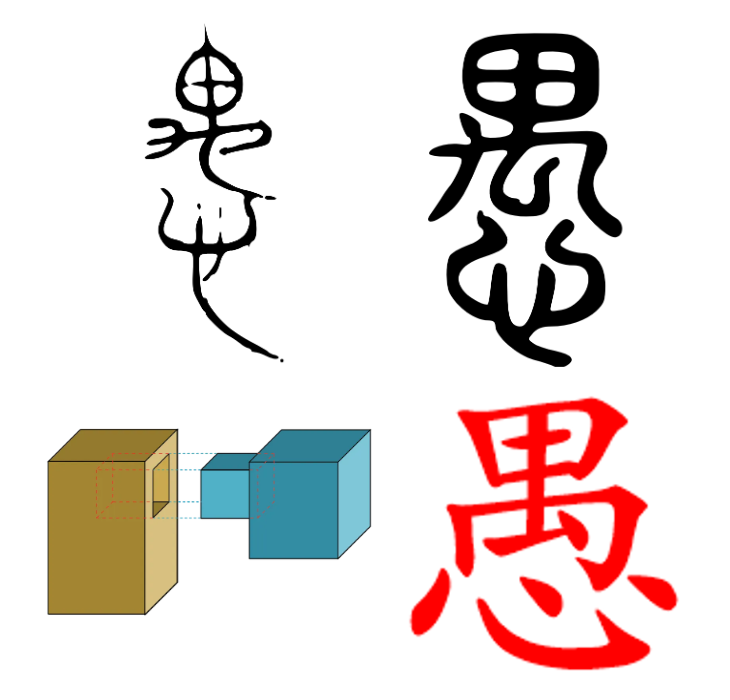
\includegraphics{./images/zi_join.png}
\caption{zi\_join}
\end{figure}

Detailed analysis of the 禺 component family demonstrates both semantic
bonding patterns and historical evolution principles:

Base Component 禺 (元字) Represents fundamental concept of
joining/coupling, analogous to a basic force carrier in physics. This
character itself is a composite: 甲 + 禸 = 禺

Derivative Characters and Their Bonding Patterns:

\begin{itemize}
\item
  亻 + 禺 = 偶 (ǒu):

  Person + joining → couple/partner

  Historical evolution: from chance meeting to deliberate pairing
\item
  宀 + 禺 = 寓 (yù):

  Roof + joining → dwelling/metaphorical connection

  Shows extension from physical to abstract space
\item
  辶 + 禺 = 遇 (yù):

  Movement + joining → encounter/meet

  Demonstrates temporal dimension of joining force
\item
  禺 + 心 = 愚 (yú):

  Heart/mind + joining → inability to make mental connections

  Reveals cognitive dimension of joining concept
\item
  阝 + 禺 = 隅 (yú):

  Wall + joining → corner/intersection

  Illustrates spatial manifestation of joining force
\item
  耒 + 禺 = 耦:

  Illustrate lotus root joining together with fibers
\end{itemize}

The semantic evolution follows predictable patterns analogous to
fundamental force interactions in physics:

\begin{itemize}
\tightlist
\item
  Spatial joining (寓, 隅): Like electromagnetic forces in physical
  space
\item
  Temporal joining (遇): Similar to weak nuclear force interactions
\item
  Conceptual joining (愚): Parallels quantum entanglement
\item
  Physical joining (偶): Resembles strong nuclear force binding
\end{itemize}

This family demonstrates how semantic forces, like physical forces,
create stable configurations that persist through time while allowing
for evolutionary adaptation to new meanings.

\hypertarget{the-ux4e4d-family}{%
\paragraph{3.3.3 The 乍 Family}\label{the-ux4e4d-family}}

\begin{figure}
\centering
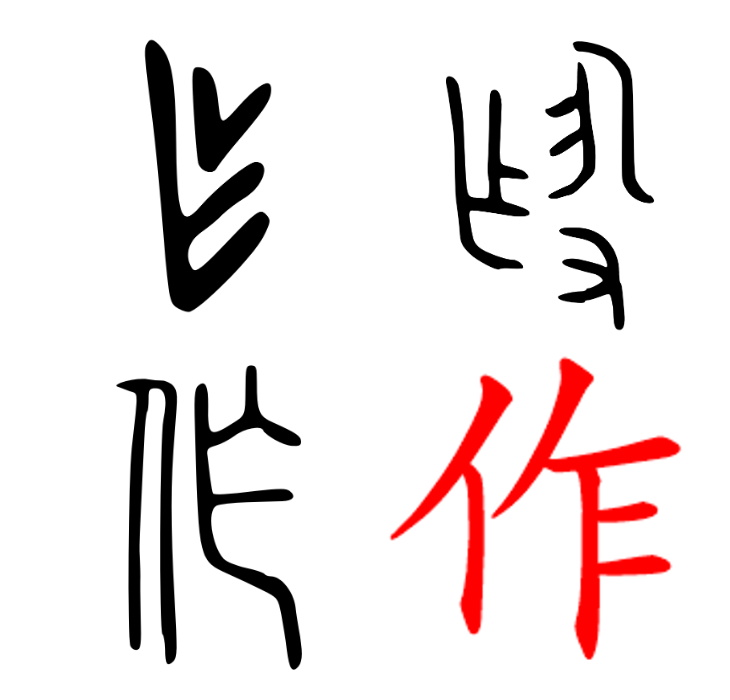
\includegraphics{./images/zi_work.png}
\caption{zi\_work}
\end{figure}

乍 means work (as both noun and verb), artifact, thing completed.

Base Component 乍 (元字)

Represents fundamental concept of work/labor, functioning as a semantic
force carrier for action and transformation

Derivative Characters and Their Bonding Patterns:

\begin{itemize}
\item
  亻 + 乍 = 作 (zuò):

  Person + work → to make/to do

  Most direct expression of the base semantic force
\item
  日 + 乍 = 昨 (zuó):

  Sun/day + work → yesterday

  Shows temporal manifestation through work completed
\item
  乍 + 心 = 怎 (zěn):

  Work + heart/mind → how?

  Represents active mental work/questioning process
\item
  火 + 乍 = 炸 (zhà):

  Fire + work → to explode/to fry

  Dual manifestation: process (cooking work) and result (explosive work)
\item
  讠 + 乍 = 诈 (zhà):

  Speech + work → to deceive

  Excessive work in communication leading to manipulation
\item
  口 + 乍 = 咋 (zǎ):

  Mouth + work → how (colloquial)

  Verbal expression of mental work/questioning
\item
  酉 + 乍 = 酢 (zuò):

  Wine + work → vinegar

  Chemical transformation through work process
\item
  ⺮ + 乍 = 笮 (zé):

  Bamboo + work → to press

  Physical work applied to materials
\item
  穴 + 乍 = 窄 (zhǎi):

  Cave/space + work → narrow

  Spatial transformation through constraining work
\end{itemize}

The semantic evolution follows patterns analogous to force interactions
in physics:

\begin{itemize}
\tightlist
\item
  Physical work (笮, 炸):
\end{itemize}

Like mechanical forces in material transformation

\begin{itemize}
\tightlist
\item
  Mental work (怎, 咋):
\end{itemize}

Parallels quantum mechanical state transitions

\begin{itemize}
\tightlist
\item
  Temporal work (昨):
\end{itemize}

Similar to time-dependent interactions

\begin{itemize}
\tightlist
\item
  Transformative work (酢, 诈):
\end{itemize}

Resembles chemical force interactions

\begin{itemize}
\tightlist
\item
  Spatial work (窄): Analogous to field effects in space
\end{itemize}

This family demonstrates how the fundamental semantic force of ``work''
combines with different contextual elements to create a rich spectrum of
meanings, from concrete physical actions to abstract temporal and mental
concepts. The systematic nature of these combinations suggests
underlying principles in character formation that mirror physical force
interactions.

The 乍 family particularly illustrates how a basic action concept can
evolve into increasingly sophisticated meanings while maintaining its
core semantic force, providing insights into both historical character
development and cognitive linguistics patterns.

\hypertarget{case-studies---pinyin---a-counter-argument}{%
\subsubsection{3.4 Case Studies - Pinyin - A
Counter-Argument}\label{case-studies---pinyin---a-counter-argument}}

While the Pinyin romanization system has undeniably augmented the
Chinese language by integrating Latin phonetic components, relying
solely on Pinyin and abandoning Chinese characters would result in a
tremendous loss. Pinyin lacks the ``character'' and personality inherent
in the logographic writing system, as many words share identical
pronunciations. In this case, character truly matters.

In the Chinese language, sound (声 shēng), form (形 xíng), and meaning
(意 yì) are all integral components of a vibrant, living system.
Overemphasizing any single aspect at the expense of the others would be
inefficient, misguided, and unwise.

To illustrate this point, consider the word ``ma''. In Pinyin, it could
represent various unrelated concepts such as 妈 (mā, mother), 马 (mǎ,
horse), or 骂 (mà, yell or curse). Without the visual distinction
provided by characters, the richness and clarity of the language would
be diminished, leading to confusion and ambiguity. Chinese characters,
in their elegance and complexity, encode both visual and auditory
information, creating a harmonious balance that has allowed the language
to flourish for millennia. Embracing and preserving this heritage, while
judiciously integrating modern enhancements like Pinyin, is the path to
ensuring the continued vitality and relevance of the Chinese language in
the 21st century and beyond.

Just as matter organizes itself into increasingly complex structures -
from atoms to molecules to molecular clusters - language exhibits
similar emergent properties at different scales. Individual characters
(字) serve as the atomic units, carrying fundamental meanings and
combining properties. These form compounds and phrases (词组), analogous
to molecules with stable semantic bonds. At a higher level of
organization, these linguistic molecules arrange themselves into
sophisticated structures like poems, which, like molecular clusters,
exhibit properties beyond the sum of their parts. This natural hierarchy
of meaning-making demonstrates the living, self-organizing nature of
Chinese language.

This self-organization manifests particularly clearly in how the
language preserves and transmits wisdom across generations. Characters
and their compounds persist not through rigid prescription but through
their resonance with human cognition and experience. Similarly,
classical poems endure not by institutional mandate but through their
ability to encode universal human insights in memorable, emotionally
resonant forms. The following case studies examine these organizing
principles at two scales: compound phrases and classical poems.

\hypertarget{case-studies---phrases-and-idioms}{%
\subsubsection{3.5 Case Studies - Phrases and
Idioms}\label{case-studies---phrases-and-idioms}}

This case study examines compound phrases containing the character 子
(zǐ) to demonstrate how network analysis reveals semantic patterns and
cognitive insights in Chinese language evolution.

\hypertarget{the-ux5b50-network-analysis}{%
\paragraph{3.5.1 The 子 Network
Analysis}\label{the-ux5b50-network-analysis}}

The character 子 exhibits remarkable semantic versatility, forming
compounds across multiple domains:

\begin{itemize}
\tightlist
\item
  Human Relations

  \begin{itemize}
  \item
    Inheritance: 子女 (children), 子孙 (descendants)
  \item
    Academic: 学子 (student), 弟子 (disciple)
  \item
    Honorific: 夫子 (master), 子 as suffix in 孔子, 老子, 墨子 (ancient
    philosophers)
  \item
    Aggressor: 洋鬼子, 毛子, 日本鬼子
  \end{itemize}
\item
  Scientific Terms

  \begin{itemize}
  \item
    Physics: 光子 (photon), 量子 (quantum), 原子 (atom), 电子
    (electron), 粒子 (particle), 分子 (molecule), 玻色子 (boson), 费米子
    (fermion)
  \item
    Biology: 孢子 (spore), 种子 (seed)
  \item
    Mathematics: 因子 (factor), 系数子 (coefficient)
  \end{itemize}
\item
  Physical Objects

  \begin{itemize}
  \item
    Tools: 筷子 (chopsticks), 梯子 (ladder)
  \item
    Containers: 箱子 (box), 瓶子 (bottle)
  \item
    Furniture: 桌子 (table), 凳子 (stool)
  \end{itemize}
\item
  Temporal Concepts

  \begin{itemize}
  \tightlist
  \item
    Time: 日子 (days/life), 子时 (midnight hour)
  \end{itemize}
\end{itemize}

\hypertarget{network-analysis-insights}{%
\paragraph{3.5.2 Network Analysis
Insights}\label{network-analysis-insights}}

Our systematic network analysis revealed a profound epistemological
insight through an unexpected discovery. Despite extensive computational
mapping of 子-compounds through both manual and automated methods, we
initially missed a crucial compound: 脑子 (brain). This oversight,
emerging during a casual walk rather than active analysis, demonstrates
a fundamental principle about knowledge systems: sometimes the most
essential elements are the hardest to see precisely because of their
foundational nature.

This discovery led to several key insights about language as a living
system:

\begin{itemize}
\tightlist
\item
  The challenge of complete enumeration in language networks

  \begin{itemize}
  \tightlist
  \item
    Even systematic approaches may miss fundamental elements
  \item
    Network completeness requires multiple analytical perspectives
  \item
    Some nodes are ``invisible'' from within the system
  \end{itemize}
\item
  The role of embodied cognition in language understanding

  \begin{itemize}
  \tightlist
  \item
    The brain studying itself faces unique epistemological challenges
  \item
    Language understanding requires both analytical and intuitive
    approaches
  \item
    Some insights emerge only through lived experience
  \end{itemize}
\item
  The limitations of purely analytical approaches

  \begin{itemize}
  \tightlist
  \item
    Computational methods, while powerful, have inherent blind spots
  \item
    The observer effect in linguistic analysis
  \item
    The need for complementary methodologies
  \end{itemize}
\end{itemize}

The missing 脑子 compound exemplifies how language evolves to encode
fundamental human experiences. This situation of late discovery in our
analysis is perfectly illustrated by the following classic poem:

\begin{verbatim}
苏轼 - 题庐山

横看成岭侧成峰,
远近高低各不同。
不识庐山真面目,
只缘身在此山中。
\end{verbatim}

(One cannot recognize the true face of Lu Mountain, Because one is
standing within it.)

Just as one cannot see the whole mountain while standing on it, our
analytical tools may miss fundamental elements precisely because they
are so intrinsic to our cognitive process. This limitation demonstrates
why network analysis must be complemented by other approaches to achieve
comprehensive understanding of linguistic structures.

Furthermore, this discovery reveals how scientific terminology emerges
and adapts within the living system of language: - Classical compounds
(like 心 for heart/mind) evolve into more specific terms (脑子 for
brain) - New scientific concepts build on existing linguistic patterns -
Language naturally develops precision while maintaining connection to
human experience

While the 子 network demonstrates how individual characters form stable
semantic compounds, an even more striking demonstration of Chinese as a
living system appears in classical poetry. Here, characters and
compounds arrange themselves into higher-order structures that achieve
remarkable efficiency in encoding human wisdom and experience. The
following analysis examines how two 20-character poems create meaning
through complementary organizing principles.

\hypertarget{case-studies---poems}{%
\subsubsection{3.6 Case Studies - Poems}\label{case-studies---poems}}

This section examines how classical Chinese poetry achieves remarkable
semantic density through minimal character usage. The survival of these
poems across millennia demonstrates powerful principles of cultural
selection, where maximum meaning with minimum structure creates enduring
linguistic configurations.

\hypertarget{plum-blossoms}{%
\paragraph{3.6.1 Plum Blossoms}\label{plum-blossoms}}

\begin{verbatim}
(I) 王安石 - 梅花

墙角数枝梅,
凌寒独自开。
遥知不是雪,
为有暗香来。
\end{verbatim}

This timeless masterpiece by Wang Anshi is a quintessential example of
classical Chinese poetry, for its ability to convey profound meaning and
beauty in 20 characters: blending artistic elegance with linguistic
efficiency to create a work that resonates across cultures and times.

\hypertarget{artistic-beauty-a-multi-sensory-experience}{%
\subparagraph{3.6.1.1 Artistic Beauty: A Multi-Sensory
Experience**}\label{artistic-beauty-a-multi-sensory-experience}}

The poem opens with a vivid image of ``a few branches of plum blossoms
by the corner of a wall'' (墙角数枝梅), their delicate white or pink
petals standing in stark contrast to the cold winter backdrop. This
visual simplicity symbolizes purity and resilience, while the ``faint
fragrance'' (暗香) of the blossoms adds an olfactory dimension, evoking
subtlety and inner virtue. The plum blossom, blooming ``alone in the
cold'' (凌寒独自开), becomes a metaphor for perseverance and moral
strength, embodying the ideals of beauty in adversity.

\hypertarget{linguistic-efficiency-depth-in-brevity}{%
\subparagraph{3.6.1.2 Linguistic Efficiency: Depth in
Brevity**}\label{linguistic-efficiency-depth-in-brevity}}

Composed of only four lines, each with five characters, the poem
demonstrates how a few carefully chosen characters can convey complex
semantics. Key characters like \textbf{梅 (plum)}, \textbf{寒 (cold)},
and \textbf{香 (fragrance)} are rich in meaning and cultural symbolism,
making them ideal for focused study. The poem's concise structure allows
learners to grasp both literal and symbolic meanings, while its vivid
imagery---such as the contrast between plum blossoms and snow---enhances
memory and comprehension.

\hypertarget{cultural-and-philosophical-resonance}{%
\subparagraph{3.6.1.3 Cultural and Philosophical
Resonance**}\label{cultural-and-philosophical-resonance}}

Rooted in Chinese cultural traditions, the plum blossom is one of the
``Four Gentlemen,'' symbolizing nobility and integrity. The poem's
philosophical depth is evident in lines like ``From afar, I know it's
not snow, because of the faint fragrance'' (遥知不是雪,为有暗香来),
which encourages readers to look beyond appearances and appreciate
subtle, enduring qualities. This universal theme of resilience and inner
beauty makes the poem accessible and meaningful to a wide audience.

\hypertarget{a-bridge-between-art-and-language}{%
\subparagraph{3.6.1.4 A Bridge Between Art and
Language**}\label{a-bridge-between-art-and-language}}

``Plum Blossoms'' is not only a masterpiece of artistic expression but
also a valuable tool for language learning. Its use of high-frequency
characters and contextual imagery provides a manageable entry point for
learners, while its cultural and philosophical layers offer deeper
insights into Chinese thought and aesthetics. The poem's minimalist
style demonstrates how simplicity can amplify impact, making it a
timeless example of the elegance and efficiency of classical Chinese
poetry.

``Plum Blossoms'' poem is a testament to the power of Chinese characters
in art and language. Through its vivid imagery, cultural symbolism, and
concise structure, the poem captures the essence of resilience, beauty,
and virtue. It serves as both a literary treasure and a linguistic gem.

\hypertarget{complementary-masterpieces-in-cultural-evolution}{%
\subparagraph{3.6.2 Complementary Masterpieces in Cultural
Evolution}\label{complementary-masterpieces-in-cultural-evolution}}

Wang Zhihuan's ``登鹳雀楼'' and Li Bai's ``静夜思'' represent perfect
exemplars of cultural survival through semantic efficiency. Each using
exactly 20 characters, these poems have persisted across twelve
centuries not through institutional preservation alone, but through
their remarkable resonance with fundamental human experiences:

\begin{verbatim}
(II) 王之涣 - 登鹳雀楼

白日依山尽,
黄河入海流。
欲穷千里目,
更上一层楼。


(III) 李白 - 静夜思

床前明月光,
疑是地上霜。
举头望明月,
低头思故乡。
\end{verbatim}

The survival of these particular poems, out of countless others written
during the Tang Dynasty, demonstrates semantic natural selection in
action. Their persistence can be attributed to several adaptive
advantages:

\begin{itemize}
\tightlist
\item
  Semantic Density: Maximum meaning in minimum space
\item
  Universal Accessibility: Basic characters carrying profound insights
\item
  Cognitive Resonance: Alignment with human thought patterns
\item
  Structural Balance: Perfect symmetry in form and meaning
\end{itemize}

\hypertarget{yin-yang-duality-in-expression}{%
\subparagraph{3.6.2.1 Yin-Yang Duality in
Expression}\label{yin-yang-duality-in-expression}}

These poems embody the Yin-Yang duality in multiple dimensions:

\begin{itemize}
\tightlist
\item
  Celestial Bodies

  \begin{itemize}
  \tightlist
  \item
    Yang (阳) Sun setting behind mountains (白日依山)
  \item
    Yin (阴): Moon casting light on earth (明月光)
  \end{itemize}
\item
  Movement Patterns

  \begin{itemize}
  \tightlist
  \item
    Yang (阳): Continuous upward progression (更上一层楼)
  \item
    Yin (阴): Circular motion of raising and lowering head
    (举头\ldots 低头)
  \end{itemize}
\item
  Philosophical Approach

  \begin{itemize}
  \tightlist
  \item
    Yang (阳): Active pursuit of transcendence through effort
  \item
    Yin (阴): Passive reception of insight through contemplation
  \end{itemize}
\item
  Emotional Register

  \begin{itemize}
  \tightlist
  \item
    Yang (阳): Aspiration toward broader horizons
  \item
    Yin (阴): Nostalgia and connection to home
  \end{itemize}
\end{itemize}

This complementarity itself represents an evolutionary advantage, as the
poems together create a complete cognitive framework for understanding
human experience - both active and contemplative approaches to wisdom.

\hypertarget{economy-of-expression-as-survival-advantage}{%
\subparagraph{3.6.2.2 Economy of Expression as Survival
Advantage}\label{economy-of-expression-as-survival-advantage}}

Both poems achieve remarkable efficiency in their use of characters:

\begin{itemize}
\tightlist
\item
  Elementary Characters

  \begin{itemize}
  \tightlist
  \item
    Basic natural elements: 山, 河, 日, 月
  \item
    Simple actions: 上, 望, 举, 低
  \item
    Fundamental concepts: 目, 光, 头, 楼
  \end{itemize}
\item
  Progressive Construction

  \begin{itemize}
  \tightlist
  \item
    From physical observation to abstract insight
  \item
    From immediate scene to expansive meaning
  \item
    From concrete details to universal themes
  \end{itemize}
\item
  Spatial Movement

  \begin{itemize}
  \tightlist
  \item
    Vertical ascent in ``登鹳雀楼''
  \item
    Circular contemplation in ``静夜思''
  \end{itemize}
\item
  Information Compression

  \begin{itemize}
  \tightlist
  \item
    Each character carries multiple layers of meaning
  \item
    Syntactic relationships multiply semantic possibilities
  \item
    Context activation maximizes cognitive engagement
  \end{itemize}
\item
  Mnemonic Efficiency

  \begin{itemize}
  \tightlist
  \item
    Rhythmic patterns aid memory
  \item
    Image patterns support recall
  \item
    Emotional resonance enhances transmission
  \end{itemize}
\end{itemize}

\hypertarget{wisdom-encoding}{%
\subparagraph{3.6.2.3 Wisdom Encoding}\label{wisdom-encoding}}

These poems demonstrate two complementary paths to wisdom:

\begin{itemize}
\tightlist
\item
  ``登鹳雀楼'': Transcendence Through Effort

  \begin{itemize}
  \tightlist
  \item
    Physical elevation as metaphor for understanding
  \item
    Continuous striving for broader perspective
  \item
    Active engagement with limitations
  \end{itemize}
\item
  ``静夜思'': Insight Through Reflection

  \begin{itemize}
  \tightlist
  \item
    Quiet observation leading to deep connection
  \item
    Natural phenomena evoking emotional truth
  \item
    Stillness revealing profound understanding
  \end{itemize}
\end{itemize}

Together, these masterpieces illustrate the remarkable capacity of
Classical Chinese to encode complex wisdom through minimal means,
achieving maximum impact through careful character selection and
arrangement.

\hypertarget{reflection-on-semantic-forces-across-scales}{%
\subsubsection{3.7 Reflection on Semantic Forces Across
Scales}\label{reflection-on-semantic-forces-across-scales}}

Our case studies reveal language as a living system shaped by semantic
forces analogous to physical forces. These forces not only bind
linguistic elements across different scales but also drive their
evolution through processes remarkably similar to biological natural
selection.

\hypertarget{hierarchy-of-semantic-bonds}{%
\paragraph{3.7.1 Hierarchy of Semantic
Bonds}\label{hierarchy-of-semantic-bonds}}

The Chinese language demonstrates organizing principles that mirror
physical systems across scales:

\begin{itemize}
\tightlist
\item
  Character Level (Atomic Scale)

  \begin{itemize}
  \tightlist
  \item
    Components bond through semantic and phonetic attraction (禺 family)
  \item
    Stable configurations emerge through cognitive resonance
  \item
    Selection pressure favors efficient meaning encoding
  \item
    Mutation and adaptation create new meanings while preserving core
    patterns
  \end{itemize}
\item
  Phrase Level (Molecular Scale)

  \begin{itemize}
  \tightlist
  \item
    Characters form compounds through semantic affinity (子-compounds)
  \item
    Stable meanings emerge from component interactions
  \item
    Successful combinations replicate across contexts
  \item
    New compounds evolve to meet changing cognitive needs
  \end{itemize}
\item
  Poetry Level (Organic Scale)

  \begin{itemize}
  \tightlist
  \item
    Characters self-organize into higher-order structures
  \item
    Emergence of properties beyond component meanings
  \item
    Selection favors maximum meaning in minimum space
  \item
    Successful forms transmit across generations
  \end{itemize}
\end{itemize}

\hypertarget{natural-selection-of-meaning}{%
\paragraph{3.7.2 Natural Selection of
Meaning}\label{natural-selection-of-meaning}}

Cultural transmission operates through selection mechanisms parallel to
biological evolution:

\begin{itemize}
\tightlist
\item
  Variation

  \begin{itemize}
  \tightlist
  \item
    Multiple expressions compete to encode similar meanings
  \item
    New combinations arise through cultural mutation
  \item
    Innovation occurs at all scales (character, phrase, poem)
  \end{itemize}
\item
  Selection

  \begin{itemize}
  \tightlist
  \item
    Efficient expressions survive (20-character poems)
  \item
    Resonant meanings propagate (classical wisdom)
  \item
    Adaptive forms emerge (scientific terminology)
  \end{itemize}
\item
  Inheritance

  \begin{itemize}
  \tightlist
  \item
    Successful patterns replicate through teaching
  \item
    Core meanings persist across cultural changes
  \item
    Adaptability enables continuous evolution
  \end{itemize}
\end{itemize}

\hypertarget{ai-enhanced-pattern-recognition}{%
\paragraph{3.7.3 AI-Enhanced Pattern
Recognition}\label{ai-enhanced-pattern-recognition}}

Modern computational approaches, particularly through AI analysis,
reveal previously invisible patterns: - Network analysis uncovers hidden
semantic relationships - Systematic mapping reveals organizational
principles - Cross-scale patterns emerge from large-scale analysis -
Human-AI collaboration bridges analytical gaps

The partnership between human insight and artificial intelligence
demonstrates how new tools can illuminate ancient patterns, revealing
the deep structure of language as a living system.

\hypertarget{ux5929ux4ebaux5408ux4e00-the-unity-of-natural-and-human-systems}{%
\paragraph{3.7.4 天人合一: The Unity of Natural and Human
Systems}\label{ux5929ux4ebaux5408ux4e00-the-unity-of-natural-and-human-systems}}

The ancient Chinese concept of 天人合一 (the unity of heaven and
humanity) finds new resonance in our analysis of semantic forces. This
principle, traditionally expressing the harmony between human and
natural worlds, now reveals itself in the parallel organizing principles
we observe across physical and linguistic domains:

\begin{itemize}
\tightlist
\item
  Self-Organization (自组)

  \begin{itemize}
  \tightlist
  \item
    Physical world: atoms → molecules → complex structures
  \item
    Language: characters → phrases → poetry
  \item
    Both: emergence of stable patterns through natural forces
  \end{itemize}
\item
  Efficiency (效率)

  \begin{itemize}
  \tightlist
  \item
    Physical world: minimum energy configurations
  \item
    Language: maximum meaning in minimal expression
  \item
    Both: optimization through natural selection
  \end{itemize}
\item
  Evolution (演化)

  \begin{itemize}
  \tightlist
  \item
    Physical world: adaptation to environmental pressures
  \item
    Language: adaptation to cognitive and cultural needs
  \item
    Both: persistent yet dynamic systems
  \end{itemize}
\end{itemize}

The bridge between sciences (天) and humanities (人) becomes
particularly visible through AI-enhanced analysis, where computational
approaches reveal patterns that transcend traditional disciplinary
boundaries. This collaboration between human insight and artificial
intelligence opens new pathways for understanding the deep unity
underlying both physical and semantic worlds.

\hypertarget{computational-pattern-discovery}{%
\subsubsection{3.8 Computational Pattern
Discovery}\label{computational-pattern-discovery}}

The computational power of ZiNets reveals fundamental structures and
relationships in Chinese characters, demonstrating deep connections
between linguistics, mathematics, and physics:

\begin{itemize}
\tightlist
\item
  Search and Analysis Framework

  \begin{itemize}
  \tightlist
  \item
    Multi-dimensional querying: Component-based, position-based, and
    pattern-based search
  \item
    Regular expression-like syntax for complex pattern matching
  \item
    Structured data representation through positional columns (zi\_left,
    zi\_mid, etc.)
  \item
    Network relationship discovery through component tracking
  \end{itemize}
\item
  Physical Analogies in Search Results

  \begin{itemize}
  \tightlist
  \item
    Component Distribution: Similar to particle distribution in quantum
    states
  \item
    Position Patterns: Analogous to preferred energy states in atomic
    structures
  \item
    Character Families: Parallel to particle families in physics
  \item
    Interaction Networks: Mirror force carrier networks in particle
    physics
  \end{itemize}
\item
  Mathematical Structure

  \begin{itemize}
  \tightlist
  \item
    Grid System: Creates a coordinate space for character composition
  \item
    Position Matrices: Track component relationships systematically
  \item
    Pattern Frequencies: Reveal statistical regularities
  \item
    Network Topology: Maps character relationship spaces
  \end{itemize}
\end{itemize}

\hypertarget{discussion-and-implications}{%
\subsection{4. Discussion and
Implications}\label{discussion-and-implications}}

\hypertarget{chinese-writing-as-a-living-system}{%
\subsubsection{4.1 Chinese Writing as a Living
System}\label{chinese-writing-as-a-living-system}}

Our computational and physics-inspired analysis reveals Chinese writing
as a living, self-organizing system that mirrors natural growth
patterns:

\begin{itemize}
\tightlist
\item
  Emergent Complexity

  \begin{itemize}
  \tightlist
  \item
    Like biological systems emerging from simple molecular interactions,
    complex characters emerge from basic 元字 combinations
  \item
    Component relationships evolve naturally based on semantic needs
  \item
    New meanings emerge through systematic combination patterns
  \item
    Character evolution follows principles of natural growth
  \end{itemize}
\item
  Self-Organization Principles

  \begin{itemize}
  \tightlist
  \item
    Characters form stable patterns without centralized design
  \item
    Component combinations follow natural efficiency principles
  \item
    Semantic relationships develop through organic usage
  \item
    System exhibits both stability and adaptability
  \end{itemize}
\item
  Natural Growth Patterns

  \begin{itemize}
  \tightlist
  \item
    Character development parallels Fibonacci patterns in nature
  \item
    Component relationships reflect natural force balances
  \item
    Evolution follows paths of least resistance
  \item
    System maintains coherence while allowing innovation
  \end{itemize}
\end{itemize}

\hypertarget{practical-implications}{%
\subsubsection{4.2 Practical
Implications}\label{practical-implications}}

\begin{itemize}
\tightlist
\item
  Understanding:

  \begin{itemize}
  \tightlist
  \item
    Characters as evolved patterns rather than arbitrary symbols
  \item
    System reflects natural organization principles
  \item
    Connection to universal growth patterns
  \item
    Evidence of semantic optimization
  \end{itemize}
\item
  Learning:

  \begin{itemize}
  \tightlist
  \item
    Focus on fundamental 元字 and their concepts
  \item
    Reduce the fundamental 元字 set to lower the entry-barrier in
    learning Chinese language. Evidently, learning 300-400 元字 first
    would be more efficient and less overwhelming than the daunting task
    of studying 3000 Chinese characters.
  \item
    Understanding natural combination patterns
  \item
    Recognition of systematic structure
  \item
    Appreciation of organic relationships
  \item
    Promote concept-based learning and break down artificial
    subject-barriers among human language, mathematics and science.
  \item
    Make STEM-oriented learning accessible to earlier ages
  \end{itemize}
\item
  Development:

  \begin{itemize}
  \tightlist
  \item
    System continues to evolve and adapt
  \item
    New characters follow established patterns
  \item
    Natural selection of effective forms
  \item
    Living language rather than static system
  \end{itemize}
\end{itemize}

\hypertarget{conclusion}{%
\subsection{5. Conclusion}\label{conclusion}}

The Chinese writing system represents a remarkable example of natural
optimization in language evolution. Through computational analysis and
theoretical reframing in terms of basic physics concepts, we reveal how:

\begin{itemize}
\tightlist
\item
  The system evolved efficient solutions for encoding meaning
\item
  Character formation follows universal organization principles
\item
  A finite set of elemental characters 元字 generates rich semantic
  expression
\item
  The system maintains stability while enabling growth
\end{itemize}

This understanding transforms our view of Chinese characters from a
designed writing system to a naturally evolved, living language system
that continues to develop according to universal principles of
organization and growth.

\hypertarget{dedication}{%
\subsection{Dedication}\label{dedication}}

This work is dedicated to late Professor T.D. Lee, whose pioneering
efforts opened doors for many Chinese students to pursue studies and
research in the United States, fostering a bridge between Eastern and
Western scientific traditions. His vision and support have enabled
countless scholars like myself to contribute to global scientific
discourse.

This work is also dedicated to author's parents, who nurtured his
intellectual curiosity through challenging times. Their sacrifices and
unwavering support are forever remembered.

\hypertarget{acknowledgements}{%
\subsection{Acknowledgements}\label{acknowledgements}}

This paper represents a collaborative effort between the author, Claude
(an AI assistant from Anthropic), and DeepSeek V3 (an AI assistant from
DeepSeek). The fusion of human knowledge in software development,
physics, and Chinese language with AI's analytical capabilities enabled
the development of the novel perspectives and methodologies presented in
this work. This collaboration demonstrates the potential of human-AI
partnerships in research, particularly in interdisciplinary studies
bridging traditional knowledge with modern computational approaches.

\hypertarget{references}{%
\subsection{References}\label{references}}

{[}1{]} https://www.wikiwand.com/en/articles/Chinese\_characters

{[}2{]} Sears, Richard. Chinese Etymology research website at
https://hanziyuan.net/

{[}3{]} Aishani Bal. The Fibonacci Series: A Hidden Order to Nature's
Designs
(https://teach-technology.org/blog/f/the-fibonacci-series-a-hidden-order-to-natures-designs)

{[}4{]} Google ImageFx text-to-image generation tool:
https://labs.google/fx/tools/image-fx

{[}5{]} 书同文 汉字网 HSK 汉语水平考试汉字列表:
https://hanzi.unihan.com.cn/School/HSK

{[}6{]} CC-CEDICT dictionary dataset :
https://www.mdbg.net/chinese/dictionary?page=cc-cedict

\hypertarget{appendix}{%
\subsection{Appendix}\label{appendix}}

\hypertarget{zinets-ux5b57ux7f51-web-app}{%
\subsubsection{ZiNets (字网) Web
App}\label{zinets-ux5b57ux7f51-web-app}}

\hypertarget{overview}{%
\paragraph{Overview}\label{overview}}

ZiNets Web App is a custom-built tool used to conduct network research
and studies on Chinese characters. It allows the author to decompose
3000 commonly used Chinese characters efficiently {[}5{]}. It also
offers search and report features. Being based in database and network
data-structure design, it enables one to discover patterns not easily
available.

It uses CC-CEDICT dataset available at MDBG free online English to
Chinese dictionary {[}6{]}.

We plan to open-source this web app in the near future. The application
visualizes and analyzes character networks using the organizational
principles described in this paper. By making this tool publicly
available, we aim to support researchers, educators, and language
enthusiasts in exploring not only Chinese characters but also other
human natural languages as naturally evolving semantic systems. The
modular design of ZiNets allows for adaptation to different writing
systems, enabling comparative studies of how various languages organize
and connect meaning through their basic elements.

\begin{itemize}
\tightlist
\item
  source code : https://github.com/digital-duck/zinets (in preparation
  for public release)
\end{itemize}

Below are a few screenshots highlighting its features.

\hypertarget{custom-built-dictionary}{%
\paragraph{Custom-built Dictionary}\label{custom-built-dictionary}}

\begin{figure}
\centering
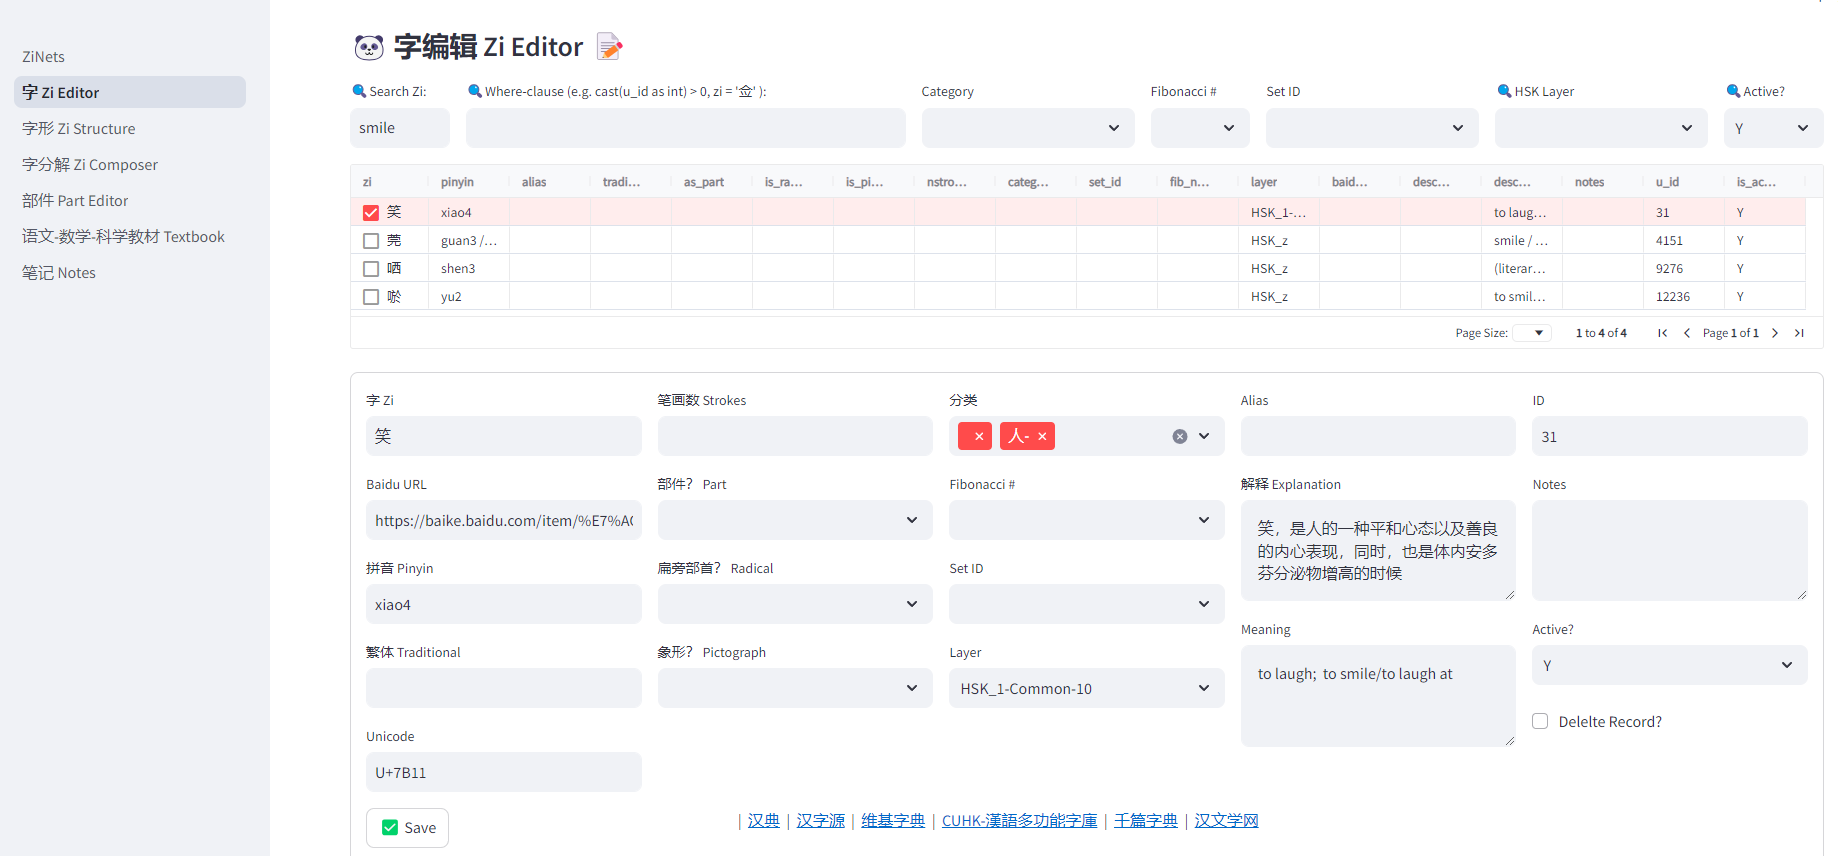
\includegraphics{./images/app_zinets.png}
\caption{ZiNets App}
\end{figure}

\hypertarget{de-compositing-characters}{%
\paragraph{De-Compositing Characters}\label{de-compositing-characters}}

\begin{figure}
\centering
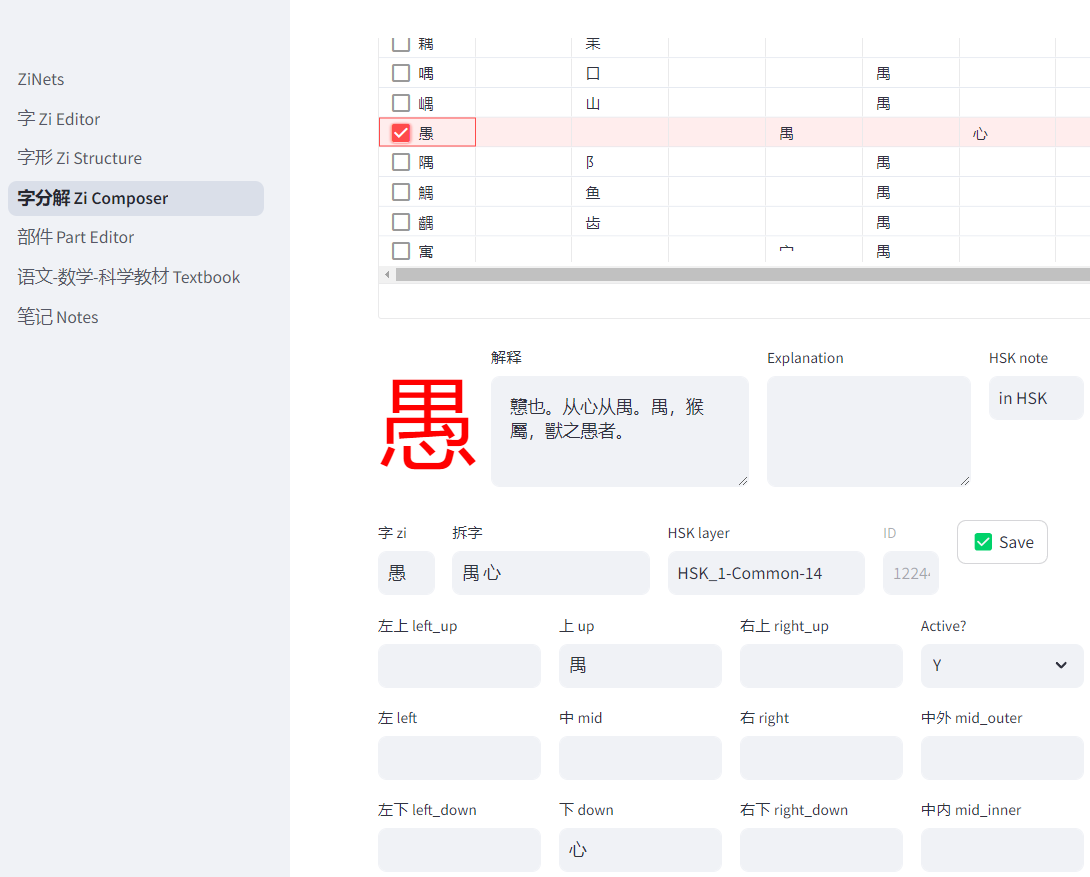
\includegraphics{./images/app_zi-parts-1.png}
\caption{Decomposition-1}
\end{figure}

\begin{figure}
\centering
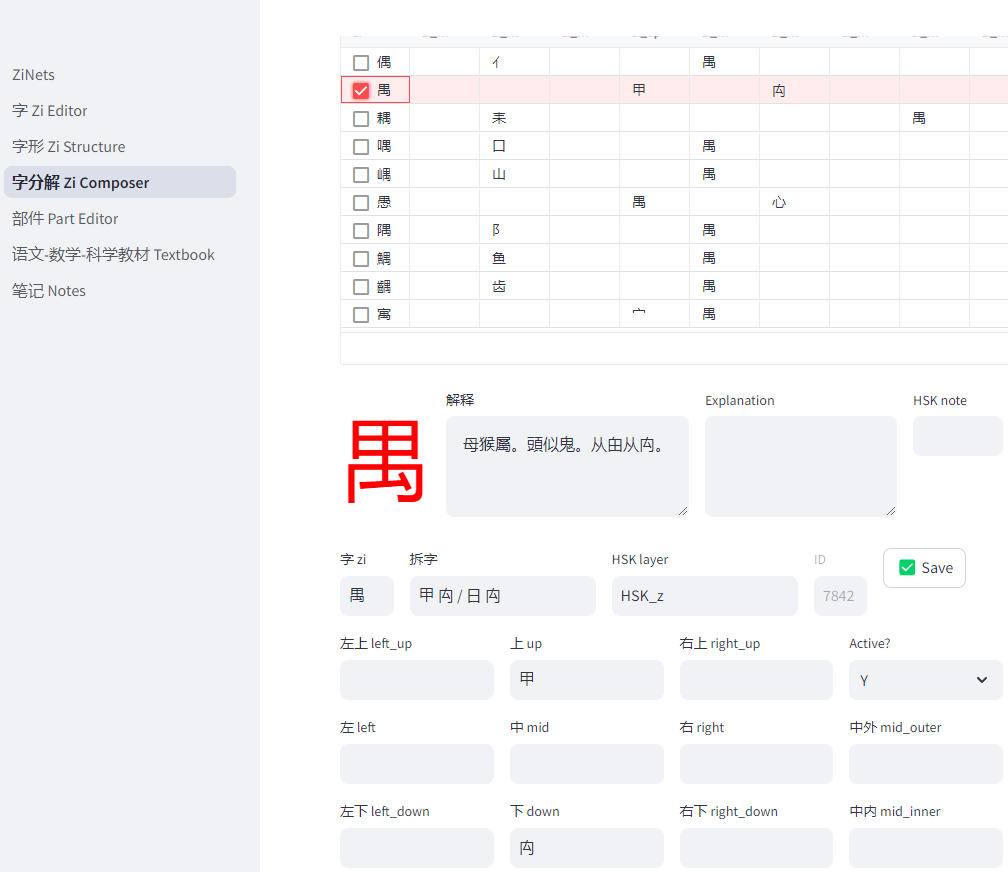
\includegraphics{./images/app_zi-parts-2.png}
\caption{Decomposition-2}
\end{figure}

\hypertarget{ux5143ux5b57-collection}{%
\paragraph{元字 Collection}\label{ux5143ux5b57-collection}}

\begin{figure}
\centering
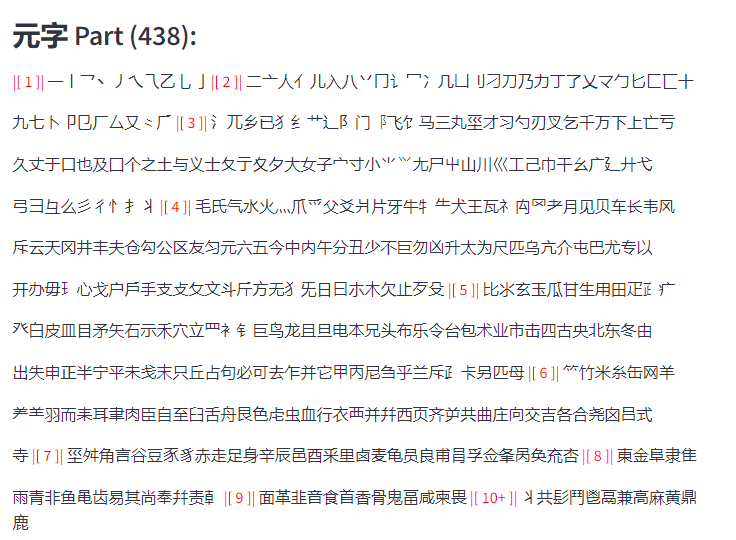
\includegraphics{./images/app_zi-elements.png}
\caption{元字 Collection}
\end{figure}

\hypertarget{search}{%
\paragraph{Search}\label{search}}

\begin{figure}
\centering
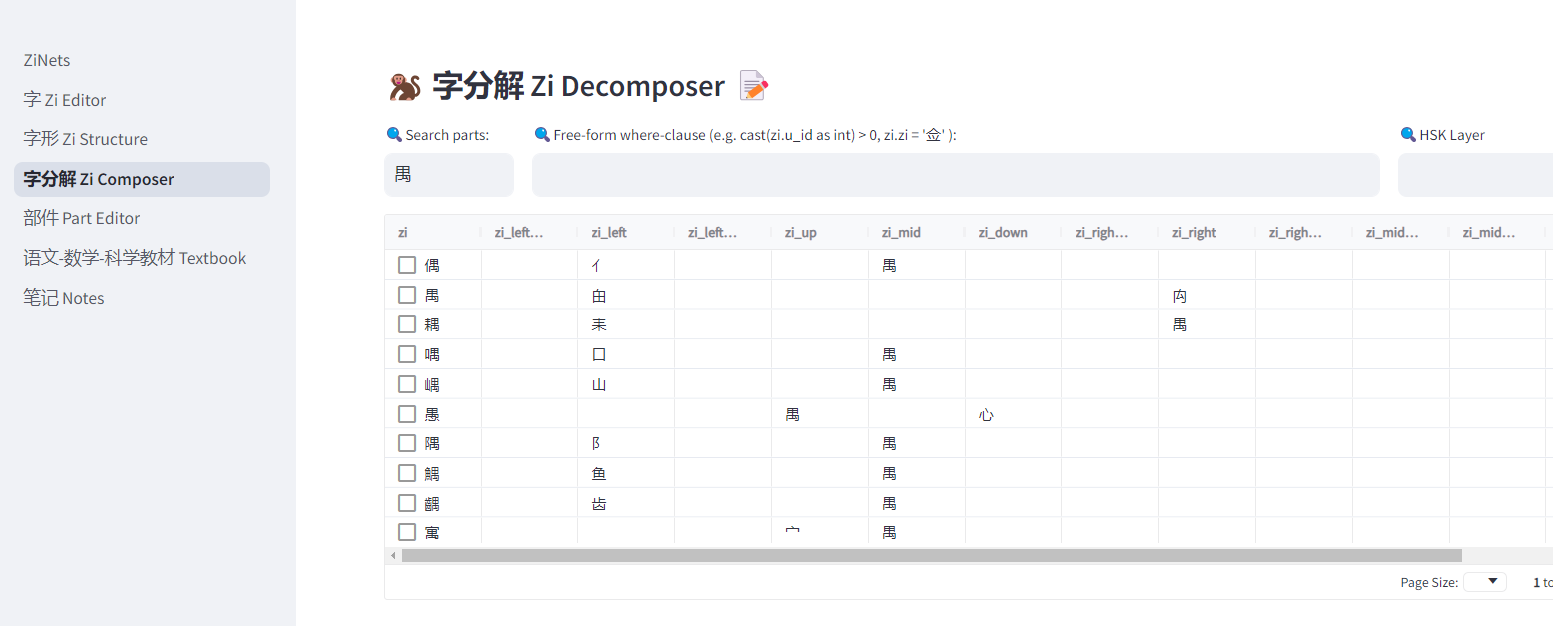
\includegraphics{./images/app_discover-zi-by-part.png}
\caption{Search Zi}
\end{figure}

\end{document}
